\documentclass[11pt]{article}
\usepackage[a4paper,margin=2cm]{geometry}
\usepackage{graphicx,booktabs,amsmath,amssymb,float,caption,subcaption}
\usepackage[hidelinks]{hyperref}
\setlength{\parskip}{4pt}\setlength{\parindent}{0pt}

\title{\textbf{PRML Lab 8 --- ICA \& Sequential Feature Selection}}
\author{Aryan Tiwari (B20AI056)\\CSL2050 Pattern Recognition \& Machine Learning, Winter 2022}
\date{}

\begin{document}
\maketitle

\section*{Question 1 --- Independent Component Analysis}

\textbf{1. Reading the audio.} The three WAV files are 6.0\,s of 16-bit audio at 44.1\,kHz (264{,}515 samples each). They are
\textbf{mutually uncorrelated} ($|r|<0.005$) and have very different distributions: excess kurtosis 2.59, $-1.50$ and 1.39, so signal 2,
the noise, is sub-Gaussian and flat-topped. These are therefore the clean independent \emph{sources}, not recordings of a mixture. Previews are
embedded in the notebook, and full-quality copies of every signal below are in \texttt{outputs/}.

\textbf{2. Creating $X$.} To merge the sources the way three microphones in one room would hear them, I scaled each source to unit
variance and mixed them as $X = AS$ with
$A=\left(\begin{smallmatrix}1&0.5&0.6\\0.6&1&0.4\\0.4&0.6&1\end{smallmatrix}\right)$ (condition number 4.3). The three mixtures are strongly
correlated ($r = 0.82$--$0.86$), and each one sounds like all three sources playing at once.

\textbf{3. ICA from scratch.}
\begin{enumerate}\itemsep0pt
\item \emph{Centring}, then \emph{whitening} with the eigen-decomposition of the covariance, $\tilde X = D^{-1/2}E^\top X$. The whitened signals are
uncorrelated with unit variance, so all that remains is to find a rotation.
\item \emph{Fixed-point update} maximising non-Gaussianity (negentropy approximated with $G(u)=\log\cosh u$):
$w \leftarrow \mathbb E[\tilde x\,\tanh(w^\top\tilde x)] - \mathbb E[1-\tanh^2(w^\top\tilde x)]\,w$, followed by normalisation.
\item \emph{Deflation}: each new $w$ is made orthogonal to the rows already found (Gram--Schmidt), so the same source is never extracted twice.
\item \emph{Convergence} as specified: stop when $|w_{new}^\top w_{old}|\approx1$ (tolerance $10^{-8}$), or after 1000 iterations.
\end{enumerate}
The three components converged in \textbf{3, 5 and 2 iterations} (0.02\,s in total), well within the 1000-iteration limit. The fixed-point update converges cubically.

\textbf{4. Mixtures, real sources and predictions.}
\begin{figure}[H]\centering
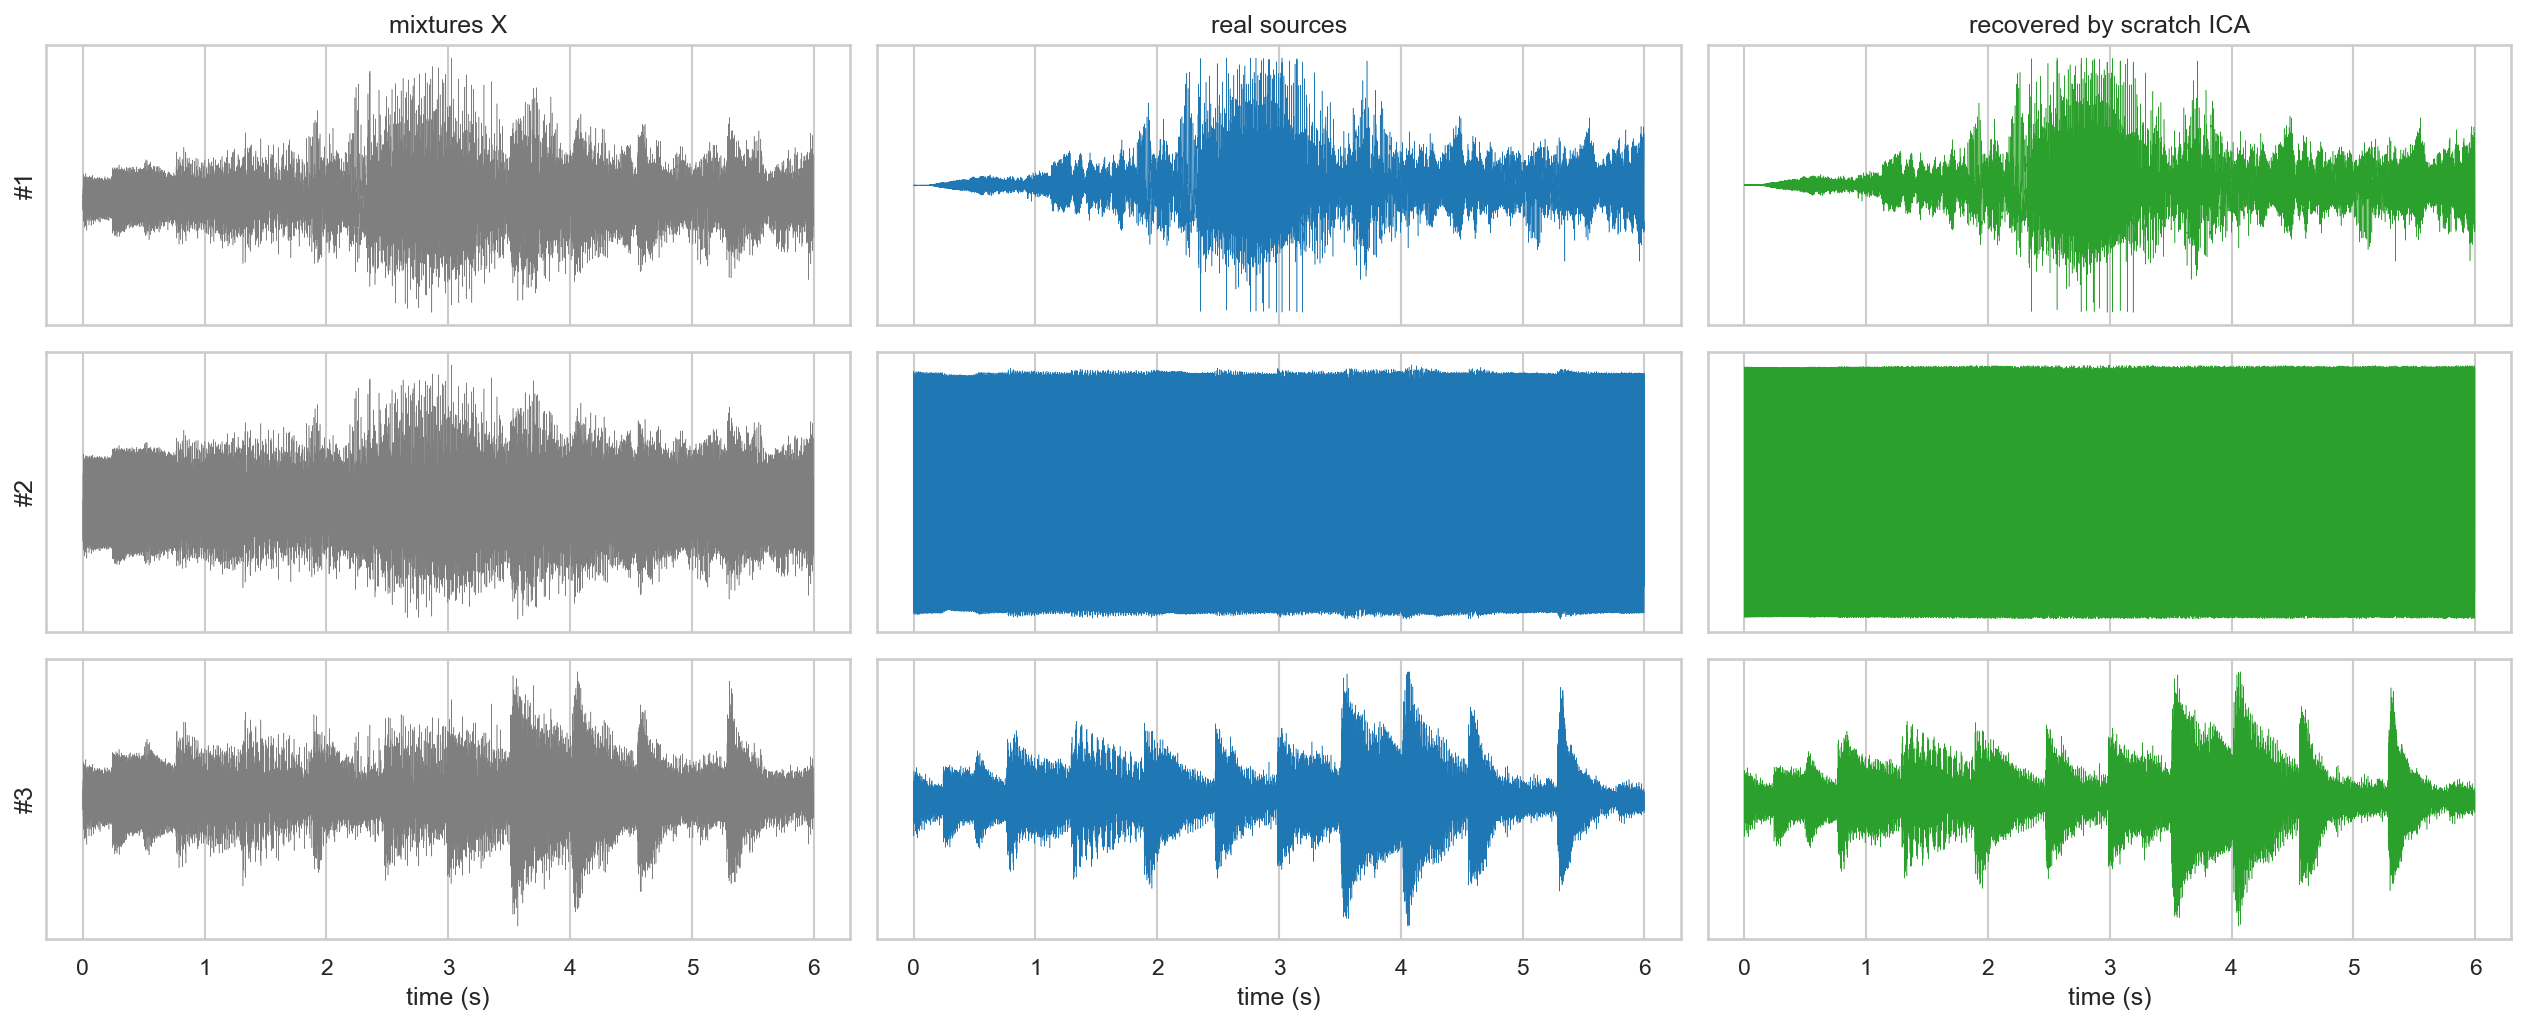
\includegraphics[width=\linewidth]{figures/q1_scratch_ica.png}
\caption{Mixtures (left), true sources (middle) and the components recovered by the scratch ICA (right), matched to sources by correlation.}
\end{figure}
\begin{figure}[H]\centering
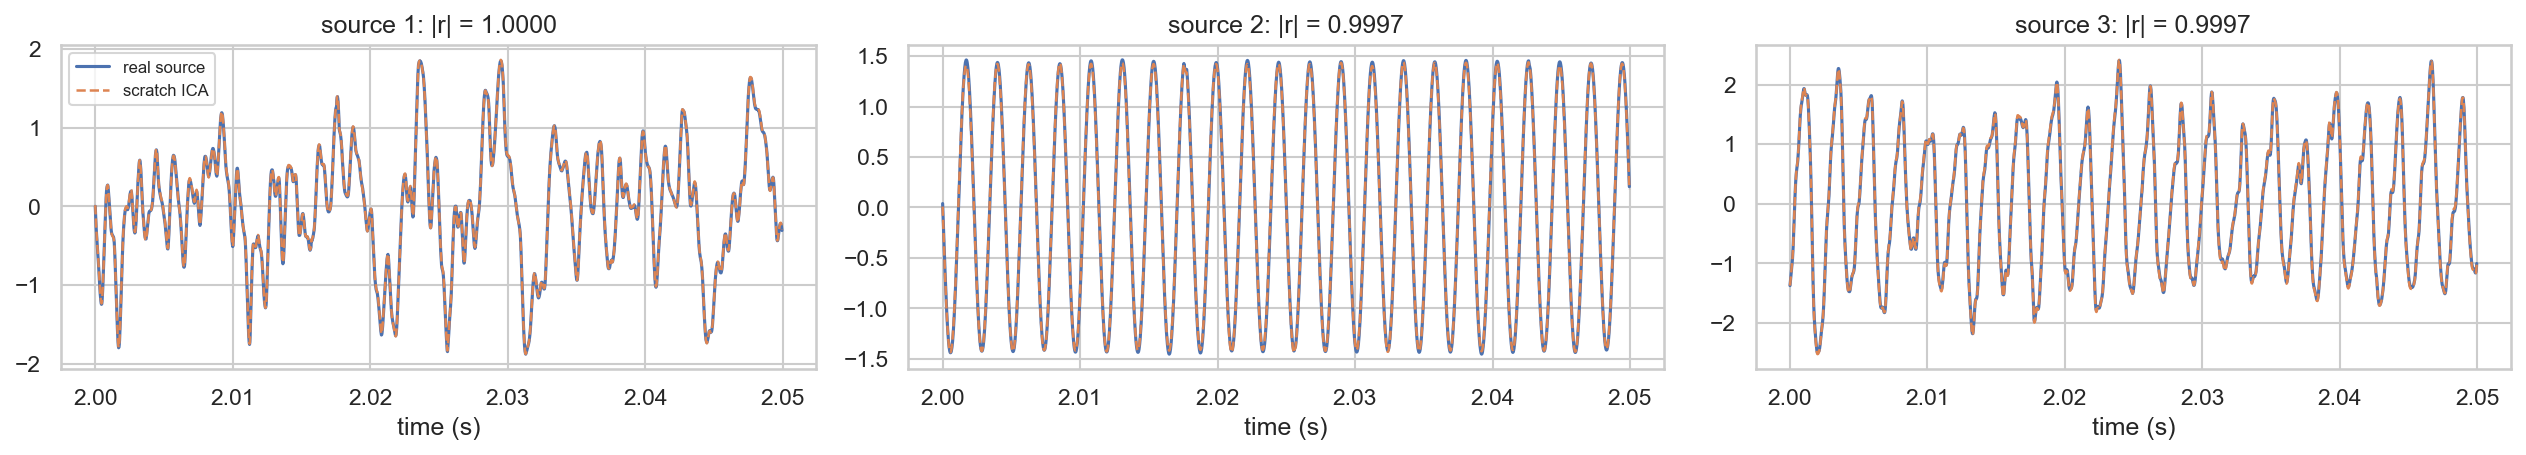
\includegraphics[width=\linewidth]{figures/q1_zoom.png}
\caption{A 50\,ms window: the recovered waveform (dashed) lies on top of the true source.}
\end{figure}

\textbf{5--6. FastICA (sklearn, 3 components).} FastICA converged in 3 iterations. Its components look and sound the same as the sources;
see \texttt{outputs/fastica\_ica\_*.wav}.

\textbf{7. Comparison.} ICA cannot recover the \emph{order}, \emph{sign} or \emph{scale} of the sources: any permutation and rescaling of $S$ explains $X$
equally well. So each output was matched to its source by the largest $|r|$, its sign was flipped if needed, and quality was measured with $|r|$
and with the signal-to-interference ratio (SIR, the energy of the correct source against the leftover energy of the others):

\begin{table}[H]\centering
\begin{tabular}{lcccc}\toprule
 & scratch $|r|$ & FastICA $|r|$ & scratch SIR (dB) & FastICA SIR (dB)\\\midrule
source 1 (piano) & 0.99995 & 0.99999 & 39.1 & 42.4\\
source 2 (noise) & 0.99971 & 0.99999 & 32.3 & 47.3\\
source 3 (music) & 0.99971 & 0.99996 & 32.4 & 40.7\\\bottomrule
\end{tabular}
\end{table}

Both methods separate the mixtures almost perfectly; the leftover interference is 30--47\,dB below the signal, which is inaudible.
The scratch and sklearn outputs correlate with each other at $|r|>0.9997$. FastICA is a few dB cleaner because it runs a tighter final
symmetric decorrelation and refines all components together, whereas my deflation scheme estimates them one at a time, so small errors in
the first components carry over into the later ones. That is why components 2 and 3 have a lower SIR than component 1 in the scratch version.
Separation works here because the sources really are independent and non-Gaussian; ICA cannot separate two Gaussian sources.

\section*{Question 2 --- Sequential Feature Selection (Airline Passenger Satisfaction)}

\textbf{1. Pre-processing.} 103{,}904 passengers, 43.3\% satisfied. \texttt{Unnamed: 0} and \texttt{id} are identifiers and were dropped.
\texttt{Arrival Delay} is missing for 310 rows; it correlates with \texttt{Departure Delay} at $r=0.965$, so each missing value was filled with
that passenger's own departure delay rather than a global median. \texttt{Gender}, \texttt{Customer Type} and \texttt{Type of Travel} were encoded as 0/1, and
\texttt{Class} as an ordinal (Eco $<$ Eco Plus $<$ Business). The ratings are already on a 0--5 scale, and a decision tree does not need scaling.
That leaves 22 features. SFS retrains the tree hundreds of times under 4-fold CV, so selection was run on a \textbf{stratified 20{,}000-row sample},
which keeps each run to a few seconds; the class balance is unchanged.

\textbf{2--3. SFS (forward, no floating, $k=10$, accuracy).} The 10 selected features reach a \textbf{4-fold CV accuracy of 93.84\%}:
\emph{Gender, Customer Type, Type of Travel, Class, Inflight wifi service, Ease of Online booking, Gate location, Online boarding,
Baggage handling, Inflight service}.

\textbf{4--6. The four configurations (cv = 4).}
\begin{table}[H]\centering
\begin{tabular}{lcccc}\toprule
Method & forward & floating & CV acc.\ (10 features) & Fold scores\\\midrule
SFS & True & False & 0.9384 & 0.940, 0.941, 0.935, 0.938\\
SBS & False & False & \textbf{0.9387} & 0.937, 0.943, 0.942, 0.934\\
SFFS & True & True & 0.9384 & same as SFS\\
SBFS & False & True & \textbf{0.9387} & same as SBS\\\bottomrule
\end{tabular}
\end{table}

\begin{figure}[H]\centering
\begin{subfigure}{0.49\linewidth}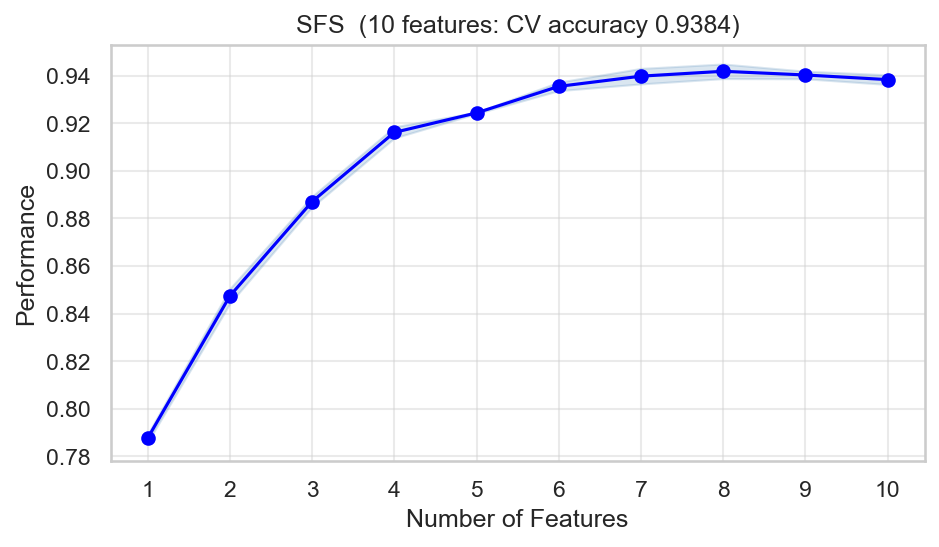
\includegraphics[width=\linewidth]{figures/q2_plot_SFS.png}\end{subfigure}
\begin{subfigure}{0.49\linewidth}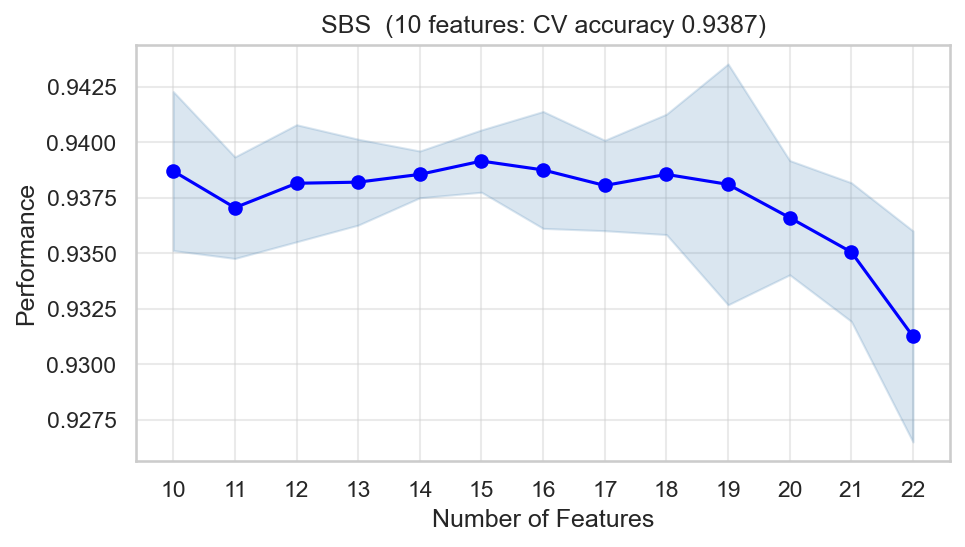
\includegraphics[width=\linewidth]{figures/q2_plot_SBS.png}\end{subfigure}\\
\begin{subfigure}{0.49\linewidth}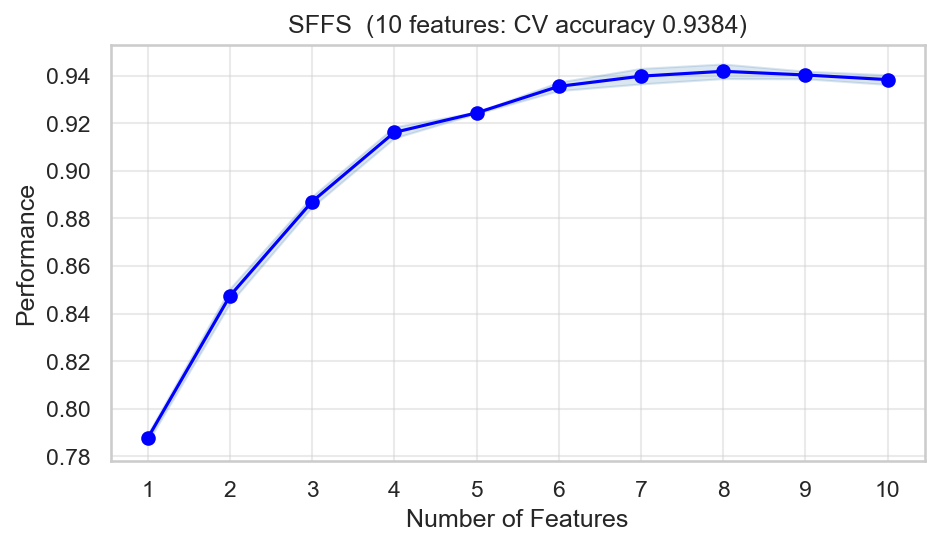
\includegraphics[width=\linewidth]{figures/q2_plot_SFFS.png}\end{subfigure}
\begin{subfigure}{0.49\linewidth}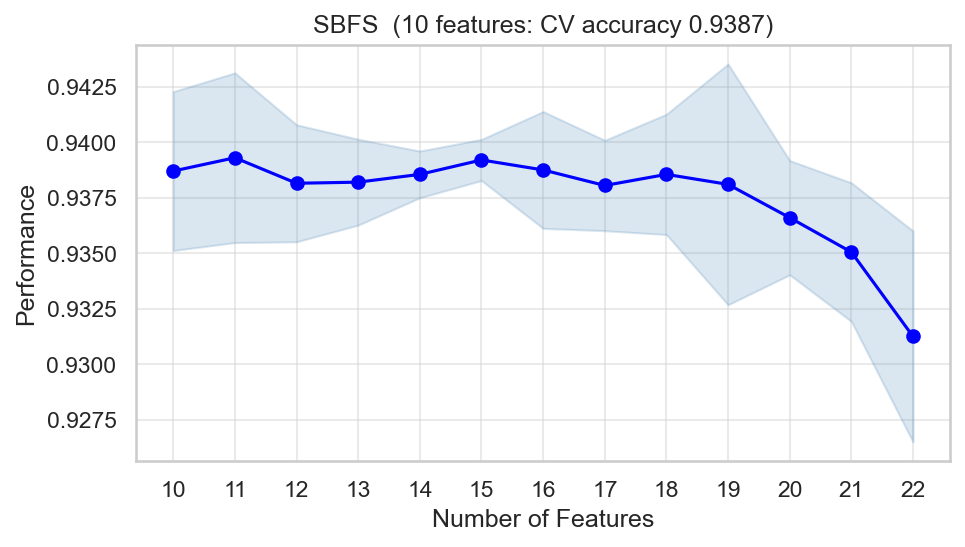
\includegraphics[width=\linewidth]{figures/q2_plot_SBFS.png}\end{subfigure}
\caption{\texttt{plot\_sequential\_feature\_selection} for each configuration (mean CV accuracy $\pm$ std at every subset size).}
\end{figure}

The full \texttt{get\_metric\_dict()} output of each run is shown as a DataFrame in the notebook. All four methods end up within 0.03 points of each other,
less than one fold's standard deviation. Floating made no difference: the conditional add/remove steps never found a swap that improved the score,
so SFFS returned the same path as SFS and SBFS the same subset as SBS. Forward and backward search differ in 3 of their 10 choices. Forward
search picked \emph{Gender, Ease of Online booking, Online boarding}; backward search kept \emph{Seat comfort, Inflight entertainment, Checkin service}. These are
mostly correlated service ratings that can stand in for one another. Seven features were chosen by all four methods: \emph{Customer Type, Type of Travel, Class,
Inflight wifi service, Gate location, Baggage handling, Inflight service}. Together they describe who is flying (loyal vs.\ new, business vs.\
personal travel, class) plus the most important service ratings.

\textbf{7. Varying the number of features.} Running forward SFS all the way to 22 features:
\begin{figure}[H]\centering
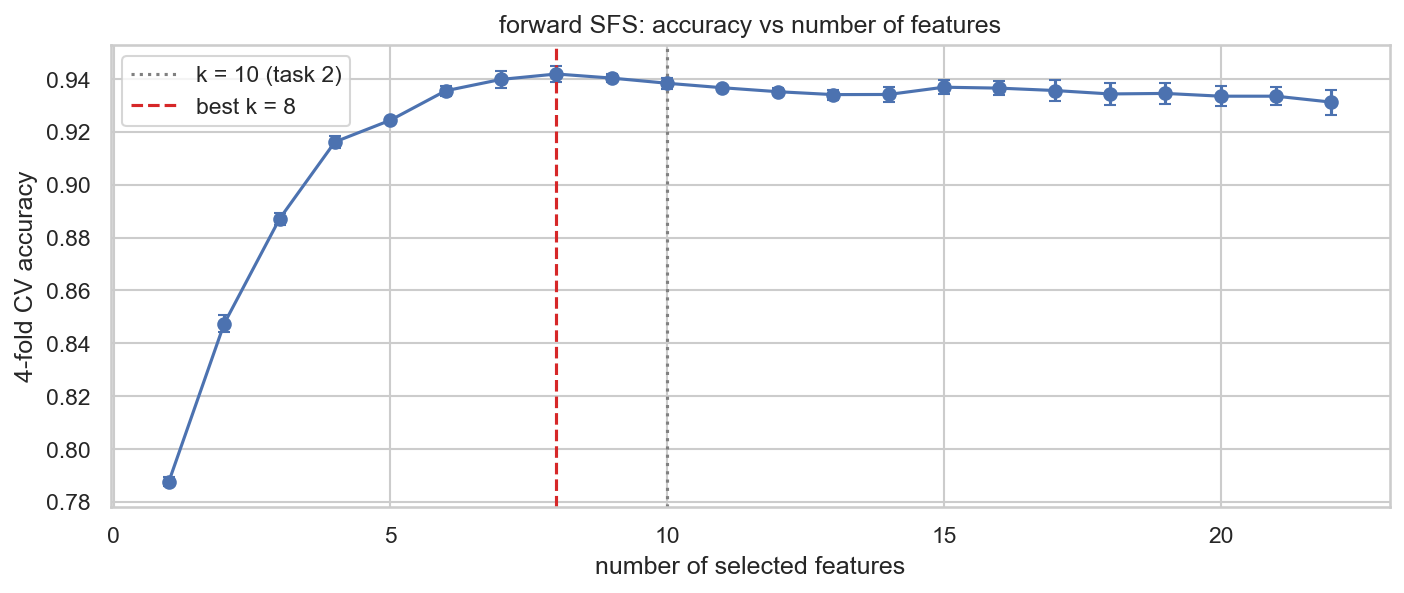
\includegraphics[width=0.85\linewidth]{figures/q2_k_curve.png}
\caption{CV accuracy as a function of the number of features selected.}
\end{figure}
Accuracy rises steeply at first. \emph{Online boarding} alone gives 78.8\%, adding \emph{Type of Travel} 84.7\%, \emph{Inflight wifi} 88.7\%, and four
features already reach 91.6\%. It peaks at \textbf{8 features (94.19\%)} and then \emph{falls slowly}, to 93.84\% at 10 and 93.12\% with all 22.
Every extra feature after the eighth gives a fully grown decision tree more ways to split on noise, so it overfits more. Asking for 10 features
is therefore slightly past the optimum. Fewer than 6 features underfits, and more than 8 adds variance without adding information.

\textbf{Bonus --- forward SFS from scratch.} At each step every remaining feature is tried with 4-fold CV and the best one is added. It picks
\textbf{exactly the same 10 features in the same order} as mlxtend. The scores are identical for the first 8 steps and differ by
$\le0.0003$ at steps 9--10. My implementation keeps the columns in selection order while mlxtend keeps them in the original order, and the
decision tree breaks ties between equally good splits by column position.

\end{document}
